\begin{sidewaysfigure}

  \begin{subfigure}{.33\linewidth}
    \centering
    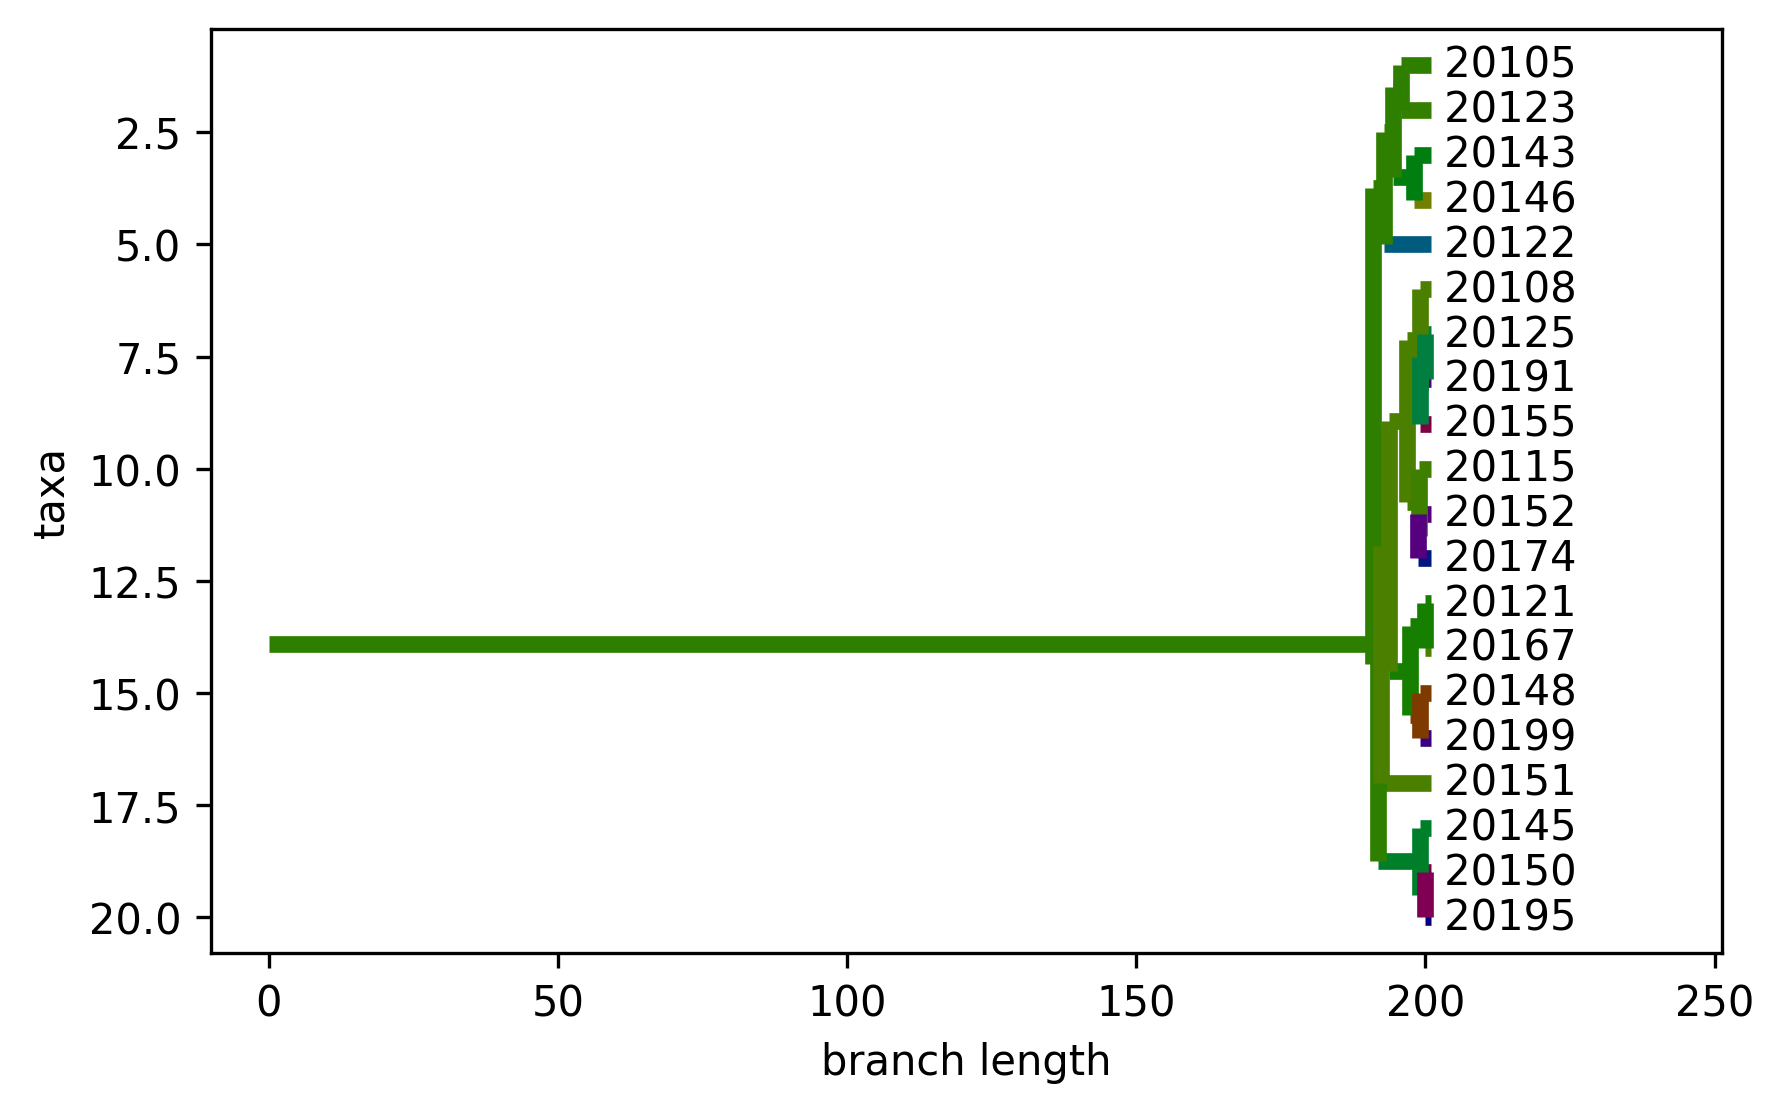
\includegraphics[width=1.05\linewidth]{notebooks/notebooks/teeplots/max_leaves=20+notebook=species-inference+replicate=0+treatment=bag+type=distilled-reference+viz=draw-biopython-tree+ext=}
    \caption{Subcaption 1}
    \label{fig:species-example-replicates:bag-reference}
  \end{subfigure}
  \begin{subfigure}{.33\linewidth}
    \centering
    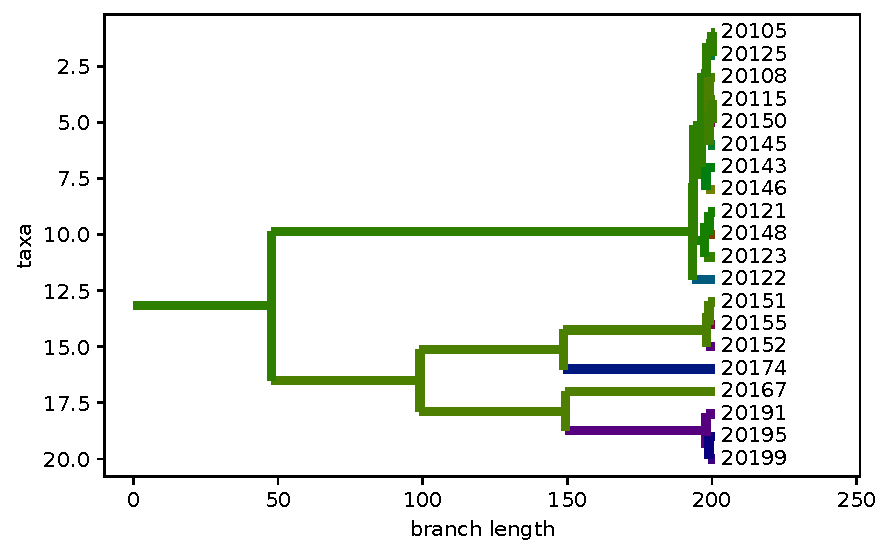
\includegraphics[width=1.05\linewidth]{notebooks/notebooks/teeplots/max_leaves=20+notebook=species-inference+replicate=0+treatment=allopatry+type=distilled-reference+viz=draw-biopython-tree+ext=}
    \caption{Allopatry reference}
    \label{fig:species-example-replicates:allopatry-reference}
  \end{subfigure}
  \begin{subfigure}{.33\linewidth}
    \centering
    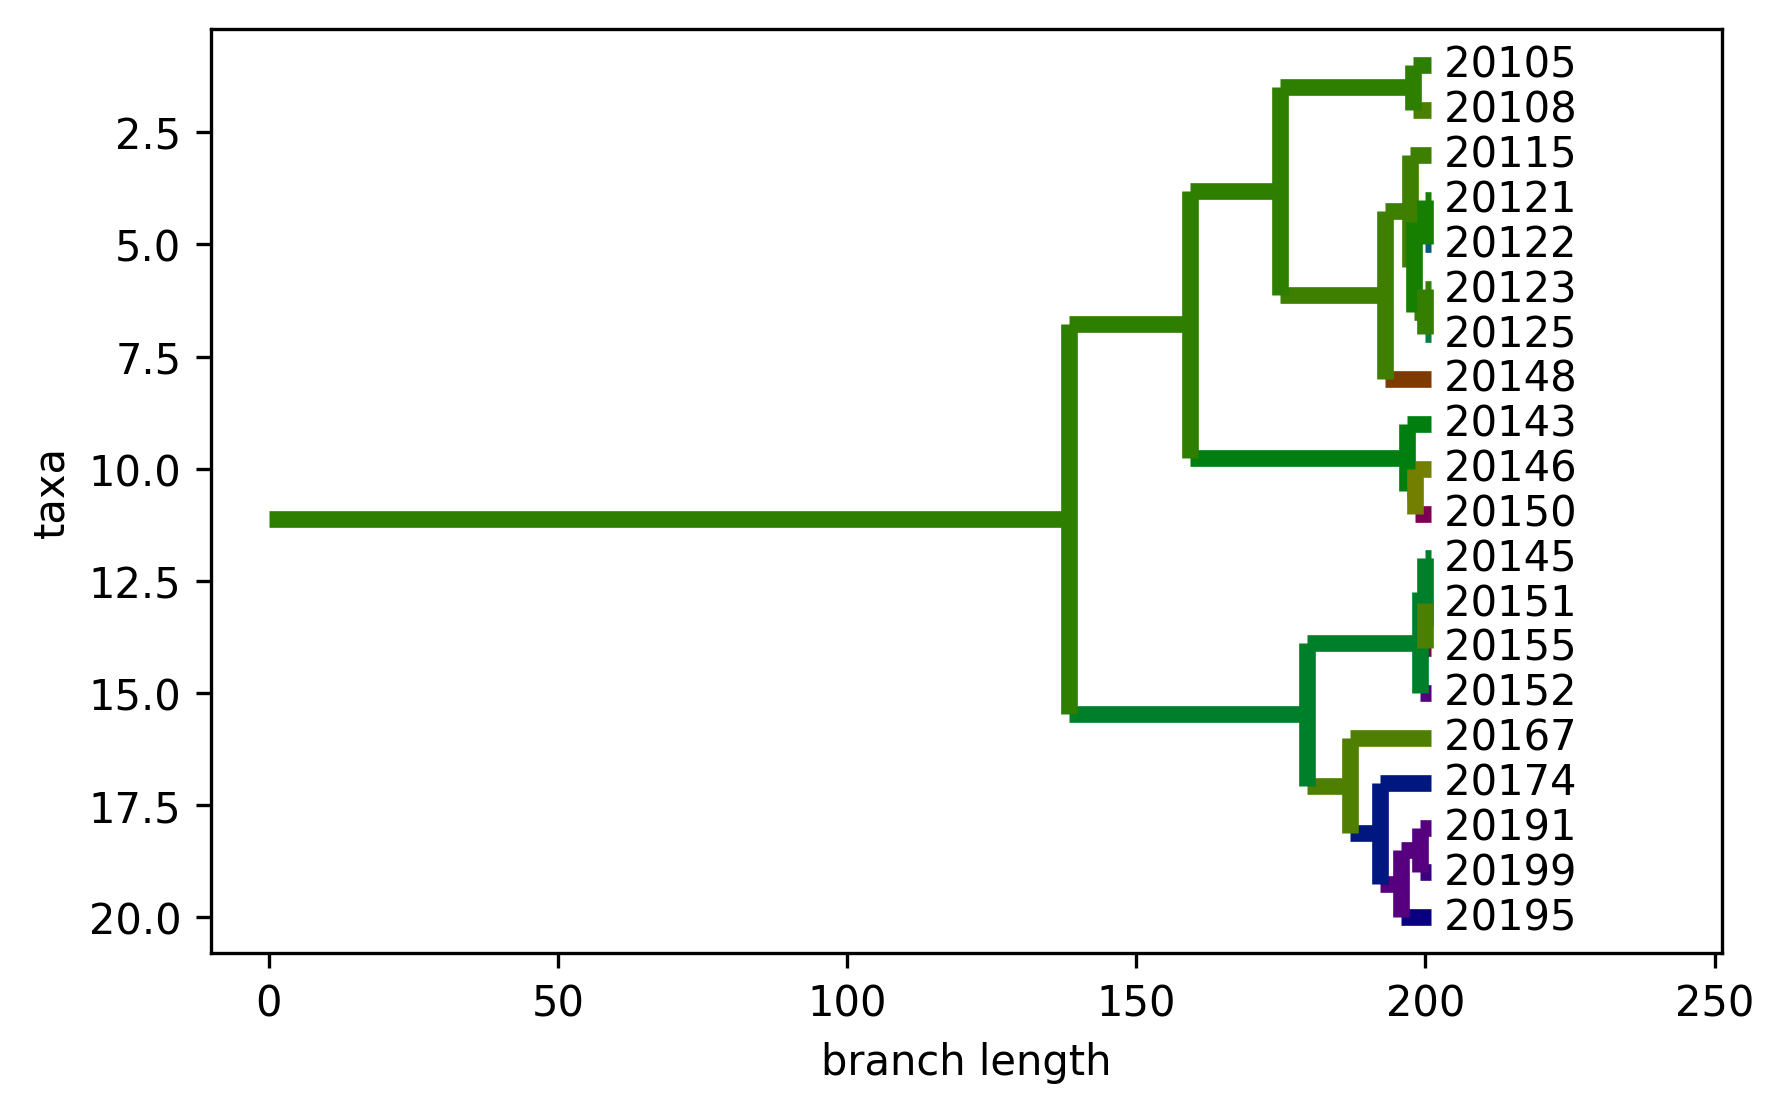
\includegraphics[width=1.05\linewidth]{notebooks/notebooks/teeplots/max_leaves=20+notebook=species-inference+replicate=0+treatment=ring+type=distilled-reference+viz=draw-biopython-tree+ext=}
    \caption{Ring reference}
    \label{fig:species-example-replicates:ring-reference}
  \end{subfigure}

  \begin{subfigure}{.33\linewidth}
    \centering
    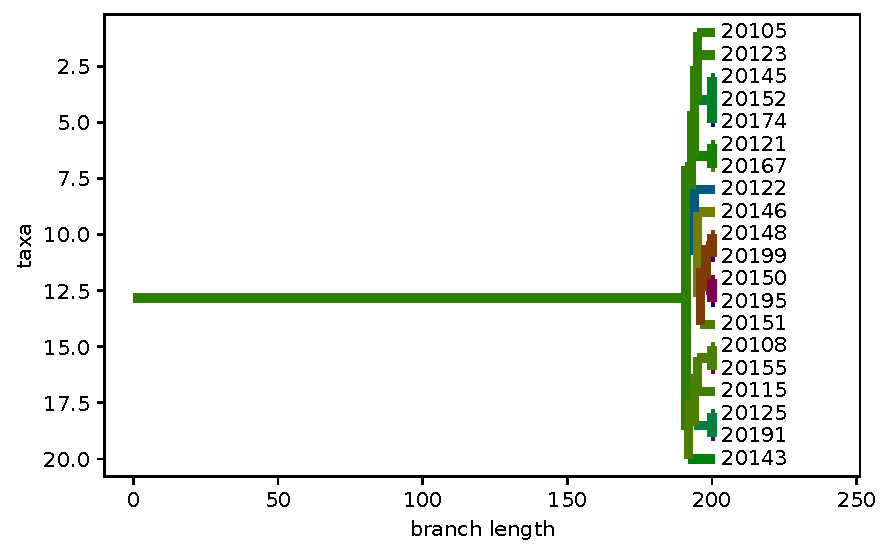
\includegraphics[width=1.05\linewidth]{notebooks/notebooks/teeplots/max_leaves=20+notebook=species-inference+replicate=0+treatment=bag+type=reconstruction+viz=draw-biopython-tree+ext=}
    \caption{Bag reconstruction}
    \label{fig:species-example-replicates:bag-reconstruction}
  \end{subfigure}
  \begin{subfigure}{.33\linewidth}
    \centering
    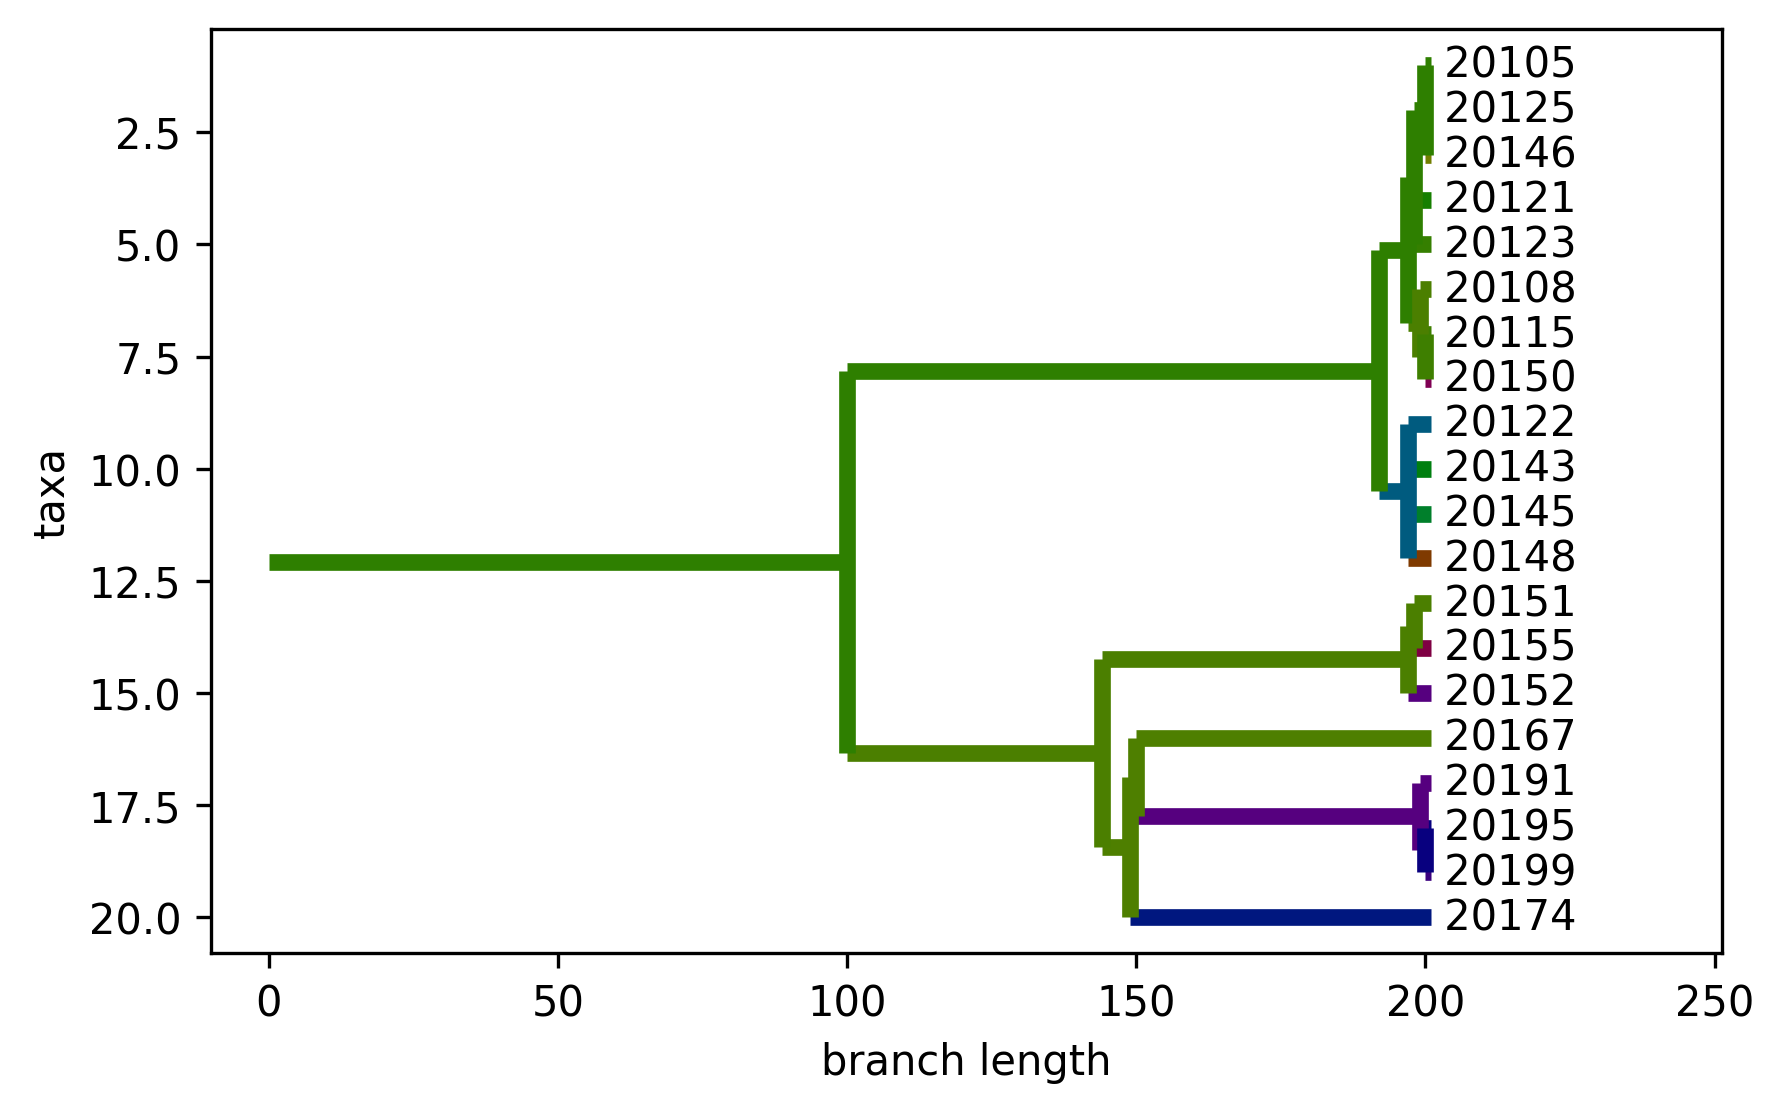
\includegraphics[width=1.05\linewidth]{notebooks/notebooks/teeplots/max_leaves=20+notebook=species-inference+replicate=0+treatment=allopatry+type=reconstruction+viz=draw-biopython-tree+ext=}
    \caption{Allopatry reconstruction}
    \label{fig:species-example-replicates:allopatry-reconstruction}
  \end{subfigure}
  \begin{subfigure}{.33\linewidth}
    \centering
    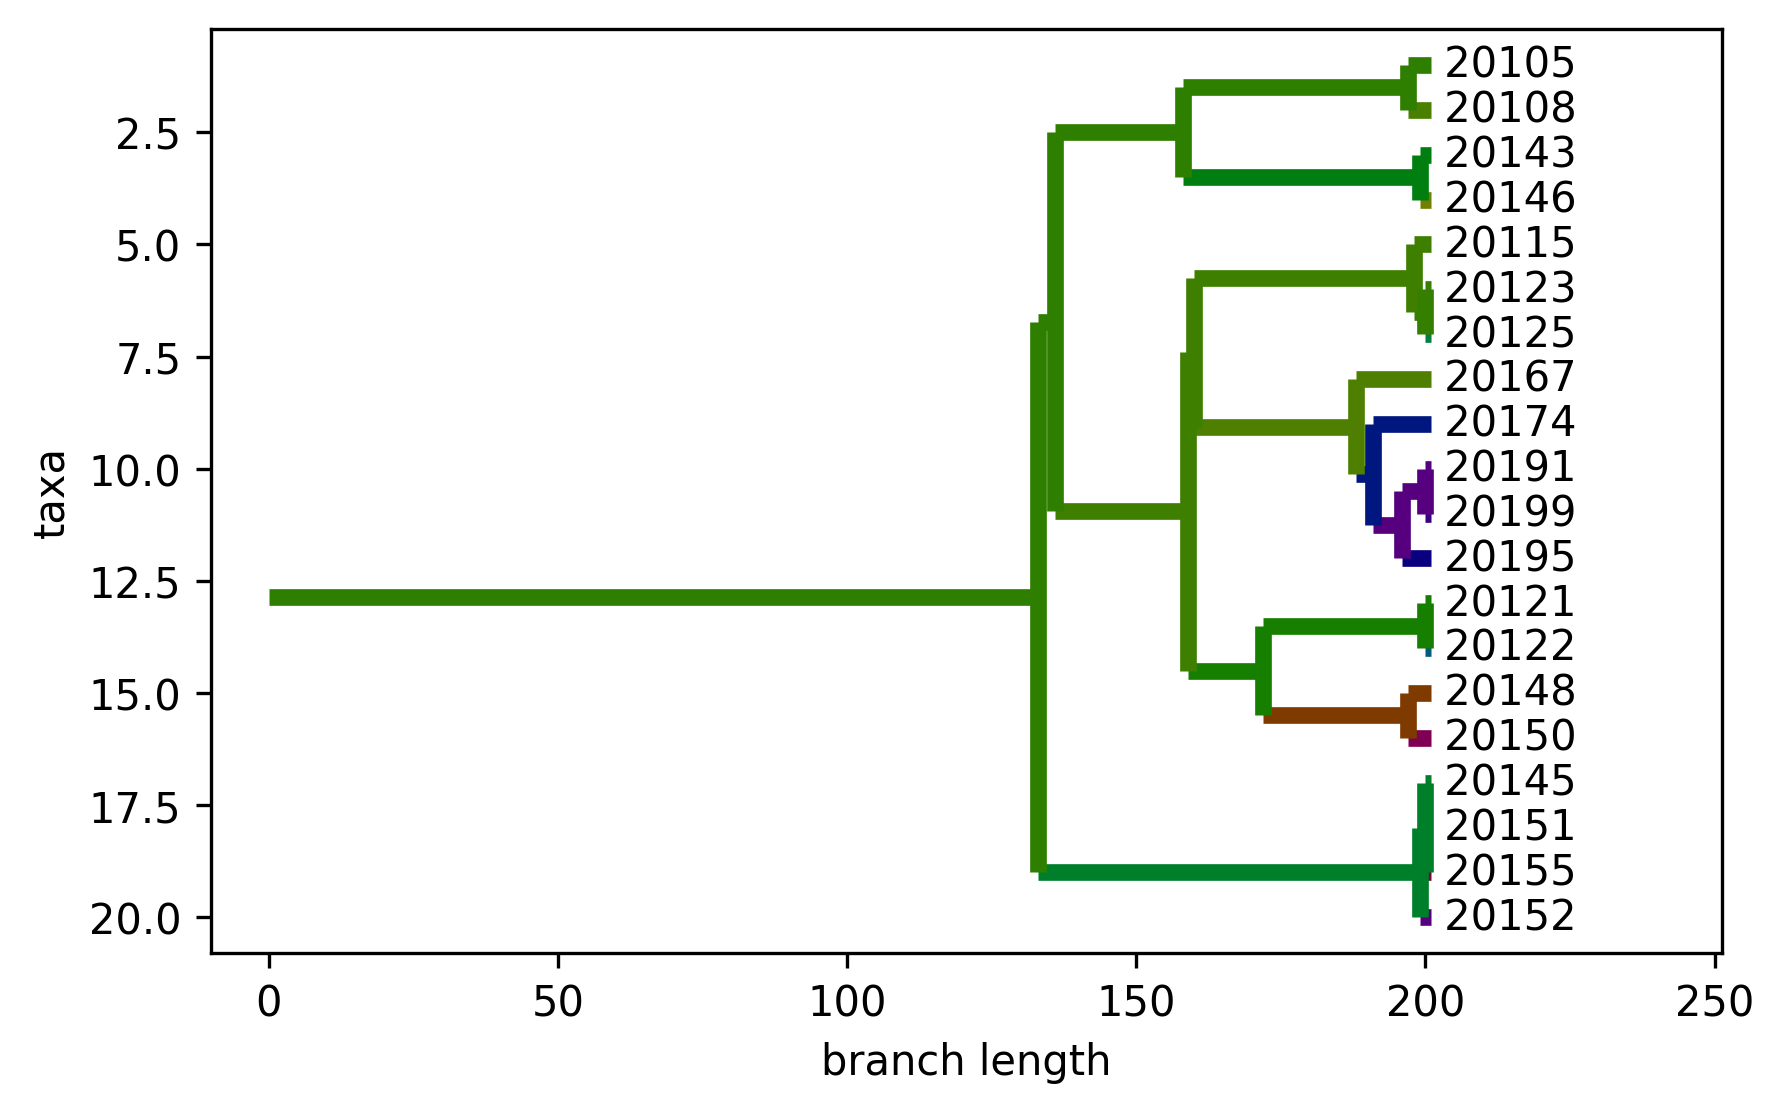
\includegraphics[width=1.05\linewidth]{notebooks/notebooks/teeplots/max_leaves=20+notebook=species-inference+replicate=0+treatment=ring+type=reconstruction+viz=draw-biopython-tree+ext=}
    \caption{Ring reconstruction}
    \label{fig:species-example-replicates:ring-reconstruction}
  \end{subfigure}

  \caption{Caption for the whole figure}
  \label{fig:species-example-replicates}

\end{sidewaysfigure}
%
% notebooks/notebooks/teeplots/max_leaves=20+notebook=species-inference+replicate=0+treatment=allopatry+type=distilled-reference+viz=draw-biopython-tree+ext=.pdf
%
% notebooks/notebooks/teeplots/max_leaves=20+notebook=species-inference+replicate=0+treatment=allopatry+type=reconstruction+viz=draw-biopython-tree+ext=.pdf
%
% notebooks/notebooks/teeplots/max_leaves=20+notebook=species-inference+replicate=0+treatment=bag+type=distilled-reference+viz=draw-biopython-tree+ext=.pdf
%
% notebooks/notebooks/teeplots/max_leaves=20+notebook=species-inference+replicate=0+treatment=bag+type=reconstruction+viz=draw-biopython-tree+ext=.pdf
%
% notebooks/notebooks/teeplots/max_leaves=20+notebook=species-inference+replicate=0+treatment=ring+type=distilled-reference+viz=draw-biopython-tree+ext=.pdf
%
% notebooks/notebooks/teeplots/max_leaves=20+notebook=species-inference+replicate=0+treatment=ring+type=reconstruction+viz=draw-biopython-tree+ext=.pdf
